\documentclass{../homework}

\title{Homework 2}
% \author{Tim Randolph}
\date{COMS W3261, Summer A 2022}

\begin{document}

\maketitle

This homework is due \textbf{Tuesday, 6/7/2022, at 11:59pm EST}. Submit to GradeScope (course code: 2KGDW8).

\textbf{Grading policy reminder:} \LaTeX~is preferred, but neatly typed or handwritten solutions are acceptable. I recommend using the .tex file for the homework as a template to write up your answers. Your TAs may dock points for indecipherable writing.\\

Proofs should be complete; that is, include enough information that a reader can clearly tell that the argument is rigorous. \\

If a question is ambiguous, please state your assumptions. This way, we can give you credit for correct work. (Even better, post on Ed so that we can resolve the ambiguity.) \\

\textbf{\LaTeX~resources.}
\begin{itemize}
    \item The website \href{https://www.overleaf.com/}{Overleaf} (essentially Google Docs for LaTeX) may make compiling and organizing your .tex files easier. Here's a quick \href{https://www.overleaf.com/learn/latex/Learn_LaTeX_in_30_minutes}{tutorial}.
    \item \href{https://detexify.kirelabs.org/classify.html}{Detexify} is a nice tool that lets you draw a symbol and returns the \LaTeX~codes for similar symbols. 
    \item The tool \href{https://www.tablesgenerator.com/}{Table Generator} makes building tables in \LaTeX~much easier.
    \item The tool \href{http://madebyevan.com/fsm/}{Finite State Machine Designer} may be useful for drawing automata. See also this example (\href{https://static.us.edusercontent.com/files/HZeTXimODzWeLvHIqsvjL2BG}{PDF}) (\href{https://static.us.edusercontent.com/files/RI3W8tQNvHMWFe9MkXV1KztA}{.tex}) of how to make fancy edges (courtesy of Eumin Hong).
    \item The website \href{https://www.mathcha.io/}{mathcha.io} allows you to draw diagrams and convert them to \LaTeX~code.
    \item To use the previous drawing tools (and for most drawing in \LaTeX), you'll need to use the package Tikz (add the command ``\textbackslash usepackage\{tikz\}'' to the preamble of your .tex file to import the package). 
    \item \href{https://www.overleaf.com/learn/latex/Positioning_of_Figures}{This tutorial} is a helpful guide to positioning figures.
\end{itemize}  

\clearpage
\section{Problem 1 (14 points)}

Examine each of the following regular expressions and write down the language it describes using set notation or 1-2 sentences. (Example: $01^+ = \{w \; | \; w $ consists of a single 0 followed by at least one 1$\}$ or ``This regular expression describes the language of strings that consist of a single 0 followed by at least one 1''.)

\begin{enumerate}
    \item (1 point.) $(00)^+ \cup (11)^+$.
    
    \item (1 point.) $a\Sigma^*a$, where $\Sigma$ denotes the alphabet $\{a, b, c\}$.
    
    \item (1 point) $(000 \cup 0000)^*$.
    
    \item (1 point) $0xHH$, where $H$ denotes the set $\{0, 1, 2, 3, 4, 5, 6, 7, 8, 9, A, B, C, D, E, F\}$ and the alphabet is $\Sigma = H \cup \{x\}$.
    
    \item (1 point) $1\big((B \cup D)(\epsilon \cup F \cup M) \cup (A \cup C)(\epsilon \cup E)\big)$, where the alphabet is 
    \[
        \Sigma = \{1, 2, 3, 4, 5, 6, A, B, C, D, E, F, G, J, L, M, N, Q, R, W, Z\}.
    \]
    
    \item (1 point) $PS0202 \cup W\big(1004 \cup 3(134 \cup 203 \cup 251 \cup 261 \cup 998) \cup 4(111 \cup 7(01 \cup 05 \cup 71) \cup 995))$, where the alphabet is $\Sigma = \{0, 1, 2, 3, 4, 5, 6, 7, 8, 9, W, P, S\}$.

\end{enumerate}

Write regular expressions that evaluate to the languages given.
\begin{enumerate}[resume]
    \item (1 point.) All strings over $\{a, b\}$, including the empty string, that can be divided into concatenated copies of the string $a$ and the string $bb$. (For example, this language includes $a$, $bbaa$, $bbbba$, and $aabba$, but not $aba$ or $babb$.)
    
    \item (2 points.) All strings over $\{a, b\}$, including the empty string, that can be divided into concatenated copies of the string $a$ and the string $bb$ \textbf{and don't contain the substring $aa$}. (For example, this language includes $a$ and $bbbba$ but not $bbaa$, $aabba$, $aba$ or $babb$.)
    
    Note that the set difference operator ($\setminus$) isn't part of our definition of a regular expression.

    \item (2 points.) Consider the alphabet $\Sigma = \{\rightarrow, \underset{0}{\rightarrow}, \underset{1}{\rightarrow}, \bigcirc, \odot\}$. Here $\rightarrow$ indicates a start symbol, $\underset{0}{\rightarrow}$ and $\underset{1}{\rightarrow}$ indicate labeled transitions, $\bigcirc$ indicates a reject state, and $\odot$ indicates an accept state. (So the string $\rightarrow \bigcirc \underset{0}{\rightarrow} \bigcirc \underset{0}{\rightarrow} \odot$ corresponds to an NFA that accepts only the string `00', and $\rightarrow \odot$ corresponds to an NFA that accepts only the string $\epsilon$.)
    
    Write a regular expression that corresponds to the language of \emph{all} NFAs that accept a single string over the alphabet $\{0, 1\}$.
    
    \item (3 points.) Write a regular expression equivalent to the language recognized by the pictured NFA, which accepts strings over $\Sigma = \{a, b, c\}$. (You can do this by converting $NFA \rightarrow DFA \rightarrow GNFA \rightarrow $ regular expression, but it will be more efficient to reason directly or take shortcuts to simplify where possible.)
    
    \begin{center}
    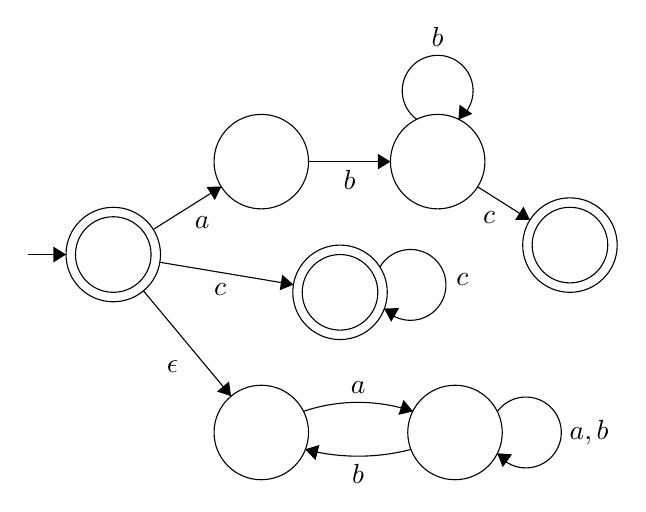
\begin{tikzpicture}[scale=0.2]
    \tikzstyle{every node}+=[inner sep=0pt]
    \draw [black] (24.8,-25.9) circle (3);
    \draw [black] (24.8,-25.9) circle (2.4);
    \draw [black] (34.2,-20) circle (3);
    \draw [black] (45.4,-20) circle (3);
    \draw [black] (53.8,-25.3) circle (3);
    \draw [black] (53.8,-25.3) circle (2.4);
    \draw [black] (39.2,-28.3) circle (3);
    \draw [black] (39.2,-28.3) circle (2.4);
    \draw [black] (34.2,-37.2) circle (3);
    \draw [black] (46.5,-37.2) circle (3);
    \draw [black] (19.4,-25.9) -- (21.8,-25.9);
    \fill [black] (21.8,-25.9) -- (21,-25.4) -- (21,-26.4);
    \draw [black] (27.34,-24.31) -- (31.66,-21.59);
    \fill [black] (31.66,-21.59) -- (30.72,-21.6) -- (31.25,-22.44);
    \draw (30.44,-23.45) node [below] {$a$};
    \draw [black] (37.2,-20) -- (42.4,-20);
    \fill [black] (42.4,-20) -- (41.6,-19.5) -- (41.6,-20.5);
    \draw (39.8,-20.5) node [below] {$b$};
    \draw [black] (44.077,-17.32) arc (234:-54:2.25);
    \draw (45.4,-12.75) node [above] {$b$};
    \fill [black] (46.72,-17.32) -- (47.6,-16.97) -- (46.79,-16.38);
    \draw [black] (47.94,-21.6) -- (51.26,-23.7);
    \fill [black] (51.26,-23.7) -- (50.85,-22.85) -- (50.32,-23.7);
    \draw (48.66,-23.15) node [below] {$c$};
    \draw [black] (41.727,-26.704) arc (150.00901:-137.99099:2.25);
    \draw (46.56,-27.5) node [right] {$c$};
    \fill [black] (42,-29.33) -- (42.45,-30.17) -- (42.95,-29.3);
    \draw [black] (27.76,-26.39) -- (36.24,-27.81);
    \fill [black] (36.24,-27.81) -- (35.53,-27.18) -- (35.37,-28.17);
    \draw (31.59,-27.69) node [below] {$c$};
    \draw [black] (26.72,-28.21) -- (32.28,-34.89);
    \fill [black] (32.28,-34.89) -- (32.15,-33.96) -- (31.39,-34.6);
    \draw (28.95,-32.99) node [left] {$\epsilon$};
    \draw [black] (36.873,-35.859) arc (108.71352:71.28648:10.838);
    \fill [black] (43.83,-35.86) -- (43.23,-35.13) -- (42.91,-36.08);
    \draw (40.35,-34.79) node [above] {$a$};
    \draw [black] (49.18,-35.877) arc (144:-144:2.25);
    \draw (53.75,-37.2) node [right] {$a,b$};
    \fill [black] (49.18,-38.52) -- (49.53,-39.4) -- (50.12,-38.59);
    \draw [black] (43.706,-38.275) arc (-75.40845:-104.59155:13.321);
    \fill [black] (36.99,-38.27) -- (37.64,-38.96) -- (37.89,-37.99);
    \draw (40.35,-39.2) node [below] {$b$};
    \end{tikzpicture}
    \end{center}
\end{enumerate}

\blfootnote{ Rationale: The goal of this question is to make sure you're comfortable interpreting and building regular expressions (and reading NFAs). }
\blfootnote{ References: Sipser pp. 63-66 (regular expressions, Lightning Review 3 (Regular Expressions); for 1.10 Sipser pp. 47-52; Lightning Review 2 (NFAs).}




\clearpage
\section{Problem 2 (6 points)}

\begin{enumerate}
    \item (6 points). Using the alphabet $\Sigma = \{o, x\}$, draw a state diagram for an NFA \textbf{with at most 4 states} that recognizes the regular expression
    \[
            (x \cup o)^*(xx \cup oo).
    \]
    Explain in words why your NFA recognizes the language specified.
        
    [Hint: Feel free to use our techniques for building NFAs that recognize languages defined with regular operations, e.g., our all-purpose method for building an NFA to recognize $A \circ B$ given NFAs that recognize $A$ and $B$. These techniques don't necessarily produce an NFA with the minimum number of states, so you may need to simplify your NFA. (Testing strings is one way to check if your simplification does the same thing as the original.)]
    
    \blfootnote{ Rationale: The goal of this question is to practice building NFAs that recognize languages defined with regular operations, and simplifying the operations of NFAs. }
    \blfootnote{ References: Sipser pp. 63-66 (NFAs), Lightning Review 2 (NFAs); Sipser pp. 59-63 (combining NFAs to recognize languages built with regular operations). }

    
\end{enumerate}

\clearpage
\section{Problem 3 (6 points)}
    \begin{enumerate}
        \item (6 points.) The DFA pictured below was created by converting from an NFA using the process described in class (also covered in video Example 2.) Work backwards to construct the original NFA and explain your reasoning. (You may assume that the original NFA has no $\epsilon$-transitions.)
        
        
        \begin{center}
        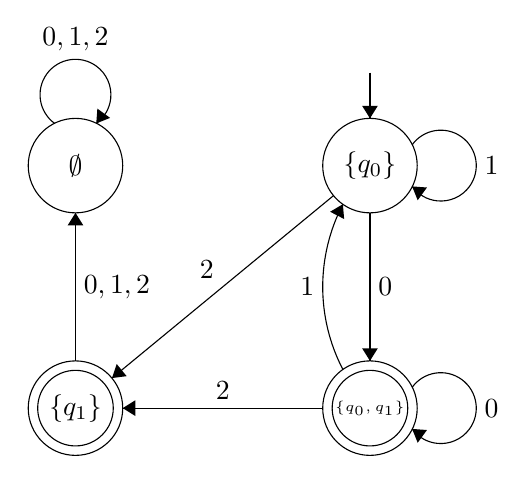
\begin{tikzpicture}[scale=0.2]
        \tikzstyle{every node}+=[inner sep=0pt]
        \draw [black] (26.7,-19.4) circle (3);
        \draw (26.7,-19.4) node {$\emptyset$};
        \draw [black] (45.4,-19.4) circle (3);
        \draw (45.4,-19.4) node {$\{q_0\}$};
        \draw [black] (26.7,-34.8) circle (3);
        \draw (26.7,-34.8) node {$\{q_1\}$};
        \draw [black] (26.7,-34.8) circle (2.4);
        \draw [black] (45.4,-34.8) circle (3);
        \draw (45.4,-34.8) node {\tiny $\{q_0,q_1\}$};
        \draw [black] (45.4,-34.8) circle (2.4);
        \draw [black] (45.4,-13.5) -- (45.4,-16.4);
        \fill [black] (45.4,-16.4) -- (45.9,-15.6) -- (44.9,-15.6);
        \draw [black] (45.4,-22.4) -- (45.4,-31.8);
        \fill [black] (45.4,-31.8) -- (45.9,-31) -- (44.9,-31);
        \draw (45.9,-27.1) node [right] {$0$};
        \draw [black] (48.08,-18.077) arc (144:-144:2.25);
        \draw (52.65,-19.4) node [right] {$1$};
        \fill [black] (48.08,-20.72) -- (48.43,-21.6) -- (49.02,-20.79);
        \draw [black] (26.7,-31.8) -- (26.7,-22.4);
        \fill [black] (26.7,-22.4) -- (26.2,-23.2) -- (27.2,-23.2);
        \draw (27.2,-27.1) node [right] {$0,1,2$};
        \draw [black] (25.377,-16.72) arc (234:-54:2.25);
        \draw (26.7,-12.15) node [above] {$0,1,2$};
        \fill [black] (28.02,-16.72) -- (28.9,-16.37) -- (28.09,-15.78);
        \draw [black] (48.08,-33.477) arc (144:-144:2.25);
        \draw (52.65,-34.8) node [right] {$0$};
        \fill [black] (48.08,-36.12) -- (48.43,-37) -- (49.02,-36.19);
        \draw [black] (43.683,-32.35) arc (-152.52527:-207.47473:11.38);
        \fill [black] (43.68,-21.85) -- (42.87,-22.33) -- (43.76,-22.79);
        \draw (41.9,-27.1) node [left] {$1$};
        \draw [black] (43.08,-21.31) -- (29.02,-32.89);
        \fill [black] (29.02,-32.89) -- (29.95,-32.77) -- (29.32,-32);
        \draw (35.04,-26.61) node [above] {$2$};
        \draw [black] (42.4,-34.8) -- (29.7,-34.8);
        \fill [black] (29.7,-34.8) -- (30.5,-35.3) -- (30.5,-34.3);
        \draw (36.05,-34.3) node [above] {$2$};
        \end{tikzpicture}
        \end{center}
    \end{enumerate}

    \blfootnote{ Rationale: The goal of this question is to practice thinking about DFAs that simulate other automata, as well as the specific process of converting an NFA into an equivalent DFA. }
    \blfootnote{ References: See Sipser pp. 54-58 (Converting DFAs to NFAs), Example 2 (Converting NFAs to DFAs). }

\clearpage
\section{Problem 4 (2 extra credit points)}
Find a cool article or paper related to theoretical computer science and write about it!

In addition to a short summary, please include why you chose the article, what you found most interesting about it, and its potential impact. Please provide a link to your chosen article or paper, and write around 300 words. The article or paper you choose does not have to be famous or revolutionary in any way. However, please do not choose a paper that you have worked on.

\end{document}
